\documentclass[a4paper, 11pt]{article}

% Nécessaire
\usepackage[french]{babel}
\usepackage[utf8]{inputenc}
\usepackage[T1]{fontenc}
\usepackage{lmodern}
\usepackage{amsmath, amsthm}
\usepackage{amsfonts,amssymb}

% Marge
\usepackage{geometry}
\geometry{margin={2.2cm ,2cm}}

% Figures, graphiques
\usepackage{graphicx}
\usepackage{epsfig}
\usepackage{caption}

% Surlignage
\usepackage{alltt}

\usepackage{xcolor}
\usepackage{soul}
\usepackage{color}
\usepackage{colortbl}

% Indicatrice
\usepackage{dsfont}

\usepackage{multirow}
\usepackage{eurosym}
\usepackage{extarrows}

% Graphique
\usepackage{tikz}


% Titre
\title{Analyse de sensibilité en prenant compte le $\mu_{\text{global}}$}
\author{}
\date{}



\begin{document}
\maketitle  

On appelle $\mu_{\text{global}}$ le produit $E \times \mu_\ell \times p_{pup} \times \frac{1}{1+SR} = 150 \times 0.04 \times 0.77 \times 0.5 = 2.31$.


L'analyse de sensibilité présentée sur la figure~\ref{fig:mug5} a été faite avec $N = 10000$ et 
\begin{itemize}
 \item $\gamma \sim \mathcal{U}[0;1]$;
 \item $p_m \sim \mathcal{U}[0;1]$;
 \item $\mu_{ER} \sim \mathcal{U}[0;1]$;
 \item $\mu_{EH} \sim \mathcal{U}[0;1]$;
 \item $k \sim \mathcal{U}[1;50]$;
 \item $\mu_{\text{global}} \sim \mathcal{U}[1;5]$.
\end{itemize}

L'analyse de sensibilité présentée sur la figure~\ref{fig:mug10} a été faite avec $N = 10000$ et 
\begin{itemize}
 \item $\gamma \sim \mathcal{U}[0;1]$;
 \item $p_m \sim \mathcal{U}[0;1]$;
 \item $\mu_{ER} \sim \mathcal{U}[0;1]$;
 \item $\mu_{EH} \sim \mathcal{U}[0;1]$;
 \item $k \sim \mathcal{U}[1;50]$;
 \item $\mu_{\text{global}} \sim \mathcal{U}[1;10]$.
\end{itemize}


\newpage


\begin{figure}[ht]
 \centering
 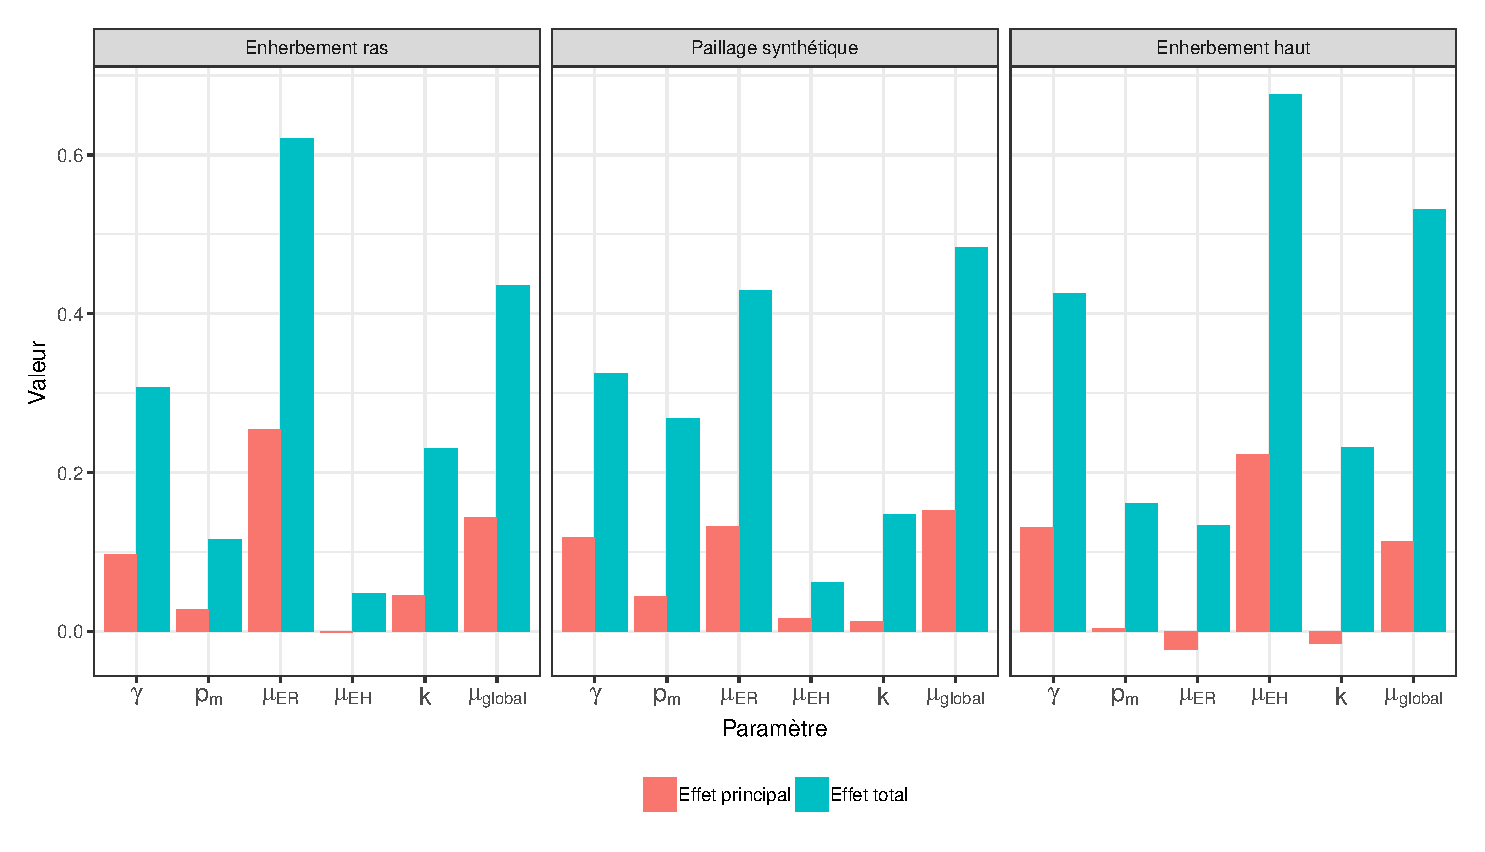
\epsfig{file = plots/sa_with_mug5.eps, scale = 0.65}
 \caption{Analyse de sensibilité avec le $\mu_{\text{global}}$ variant entre 1 et 5.}
 \label{fig:mug5}
\end{figure}


\begin{figure}[!h]
 \centering
 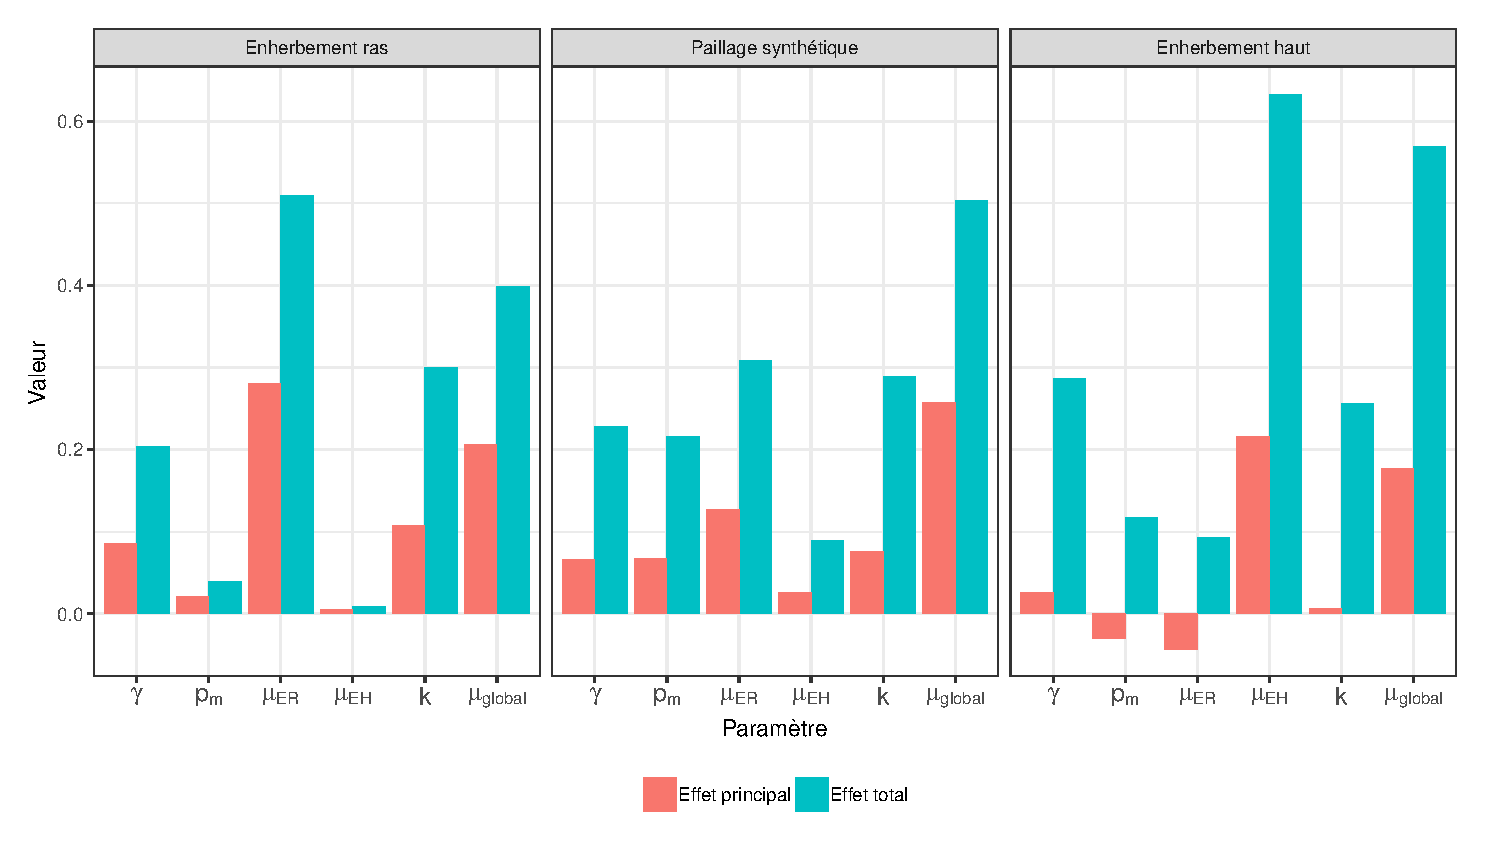
\epsfig{file = plots/sa_with_mug10.eps, scale = 0.65}
 \caption{Analyse de sensibilité avec le $\mu_{\text{global}}$ variant entre 1 et 10.}
 \label{fig:mug10}
\end{figure}




\end{document}

